\section{Opgave 3 - Guess a HEX number game}
\begin{enumerate}
	\item[1)]
	Vi skriver koden for vores Guessgame som det ses på figur \ref{lst:Guessgame}.\\
	\begin{lstlisting}[caption={Behavioral style kode for Guessgame},label={lst:Guessgame}]
library ieee;
use ieee.std_logic_1164.all;
use ieee.numeric_std.all;

entity guessgame is 
port (input : in std_logic_vector(7 downto 0);
set, show, try : in std_logic;
seg1, seg10 : out std_logic_vector(6 downto 0));
end guessgame;

architecture game_process of guessgame is
signal i_input10 : std_logic_vector(7 downto 4);
signal i_input1 : std_logic_vector(3 downto 0);
signal i_seg1, i_seg10 : std_logic_vector(3 downto 0);
begin
count: process (set, show, try)

variable target : std_logic_vector(7 downto 0);

begin

--target := "00000000";

if set = '0' then target := input;
elsif show = '0' then 
i_seg1 <= target(3 downto 0);
i_seg10 <= target(7 downto 4);
case i_seg1 is
when "0000" => seg1 <= "0000001"; -- 0
when "0001" => seg1 <= "1001111"; -- 1
when "0010" => seg1 <= "0010010"; -- 2
when "0011" => seg1 <= "0000110"; -- 3
when "0100" => seg1 <= "1001100"; -- 4
when "0101" => seg1 <= "0100100"; -- 5
when "0110" => seg1 <= "0100000"; -- 6
when "0111" => seg1 <= "0001111"; -- 7
when "1000" => seg1 <= "0000000"; -- 8
when "1001" => seg1 <= "0001100"; -- 9
when "1010" => seg1 <= "0001000"; -- A
when "1011" => seg1 <= "1100000"; -- B
when "1100" => seg1 <= "0110001"; -- C
when "1101" => seg1 <= "1000010"; -- D
when "1110" => seg1 <= "0110000"; -- E
when "1111" => seg1 <= "0111000"; -- F
when others => seg1 <= "1111111"; -- Slukket
end case;
case i_seg10 is
when "0000" => seg10 <= "0000001"; -- 0
when "0001" => seg10 <= "1001111"; -- 1
when "0010" => seg10 <= "0010010"; -- 2
when "0011" => seg10 <= "0000110"; -- 3
when "0100" => seg10 <= "1001100"; -- 4
when "0101" => seg10 <= "0100100"; -- 5
when "0110" => seg10 <= "0100000"; -- 6
when "0111" => seg10 <= "0001111"; -- 7
when "1000" => seg10	<= "0000000"; -- 8
when "1001" => seg10	<= "0001100"; -- 9
when "1010" => seg10 <= "0001000"; -- A
when "1011" => seg10 <= "1100000"; -- B
when "1100" => seg10 <= "0110001"; -- C
when "1101" => seg10	<= "1000010"; -- D
when "1110" => seg10 <= "0110000"; -- E
when "1111" => seg10 <= "0111000"; -- F
when others => seg10 <= "1111111"; -- Slukket
end case;
elsif try = '0' then 
if input > target then --output Hi
seg10 <= "1001000"; 
seg1 <= "1111001";
elsif input < target then -- output Lo
seg10 <= "1110001"; 
seg1 <= "1100010";
elsif input = target then -- output --
seg10 <= "1111110"; 
seg1 <= "1111110";
end if;
elsif set = '1' and show = '1' and try = '1' then 
i_input10 <= input(7 downto 4); 
i_input1 <= input(3 downto 0);
case i_input1 is
when "0000" => seg1 <= "0000001"; -- 0
when "0001" => seg1 <= "1001111"; -- 1
when "0010" => seg1 <= "0010010"; -- 2
when "0011" => seg1 <= "0000110"; -- 3
when "0100" => seg1 <= "1001100"; -- 4
when "0101" => seg1 <= "0100100"; -- 5
when "0110" => seg1 <= "0100000"; -- 6
when "0111" => seg1 <= "0001111"; -- 7
when "1000" => seg1 <= "0000000"; -- 8
when "1001" => seg1 <= "0001100"; -- 9
when "1010" => seg1 <= "0001000"; -- A
when "1011" => seg1 <= "1100000"; -- B
when "1100" => seg1 <= "0110001"; -- C
when "1101" => seg1 <= "1000010"; -- D
when "1110" => seg1 <= "0110000"; -- E
when "1111" => seg1 <= "0111000"; -- F
when others => seg1 <= "1111111"; -- Slukket
end case;

case i_input10 is
when "0000" => seg10 <= "0000001"; -- 0
when "0001" => seg10 <= "1001111"; -- 1
when "0010" => seg10 <= "0010010"; -- 2
when "0011" => seg10 <= "0000110"; -- 3
when "0100" => seg10 <= "1001100"; -- 4
when "0101" => seg10 <= "0100100"; -- 5
when "0110" => seg10 <= "0100000"; -- 6
when "0111" => seg10 <= "0001111"; -- 7
when "1000" => seg10 <= "0000000"; -- 8
when "1001" => seg10 <= "0001100"; -- 9
when "1010" => seg10 <= "0001000"; -- A
when "1011" => seg10 <= "1100000"; -- B
when "1100" => seg10 <= "0110001"; -- C
when "1101" => seg10 <= "1000010"; -- D
when "1110" => seg10 <= "0110000"; -- E
when "1111" => seg10 <= "0111000"; -- F
when others => seg10 <= "1111111"; -- Slukket
end case;
end if;
end process count;
end game_process;


	\end{lstlisting}
	\item[2)]
	Vi downloader programmet til vores DE2-board, hvor SW[0-3] vises på HEX0, SW[4-7] vises på HEX1, KEY3 = set, KEY2 = show og KEY1 = try. \\
	\begin{figure}[h]
		\centering
		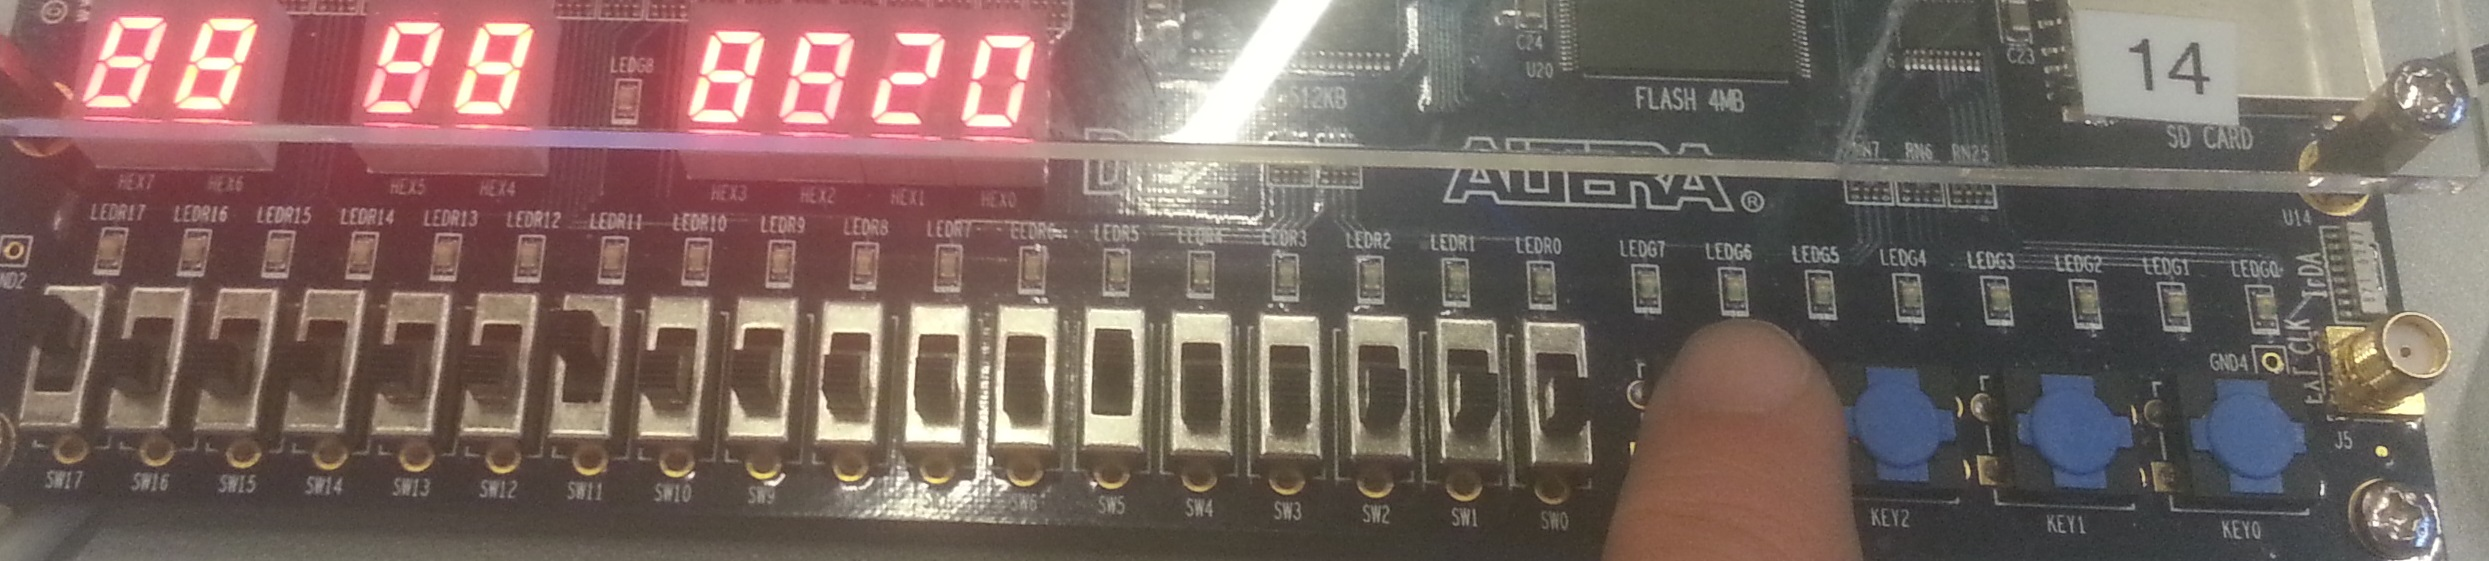
\includegraphics[scale=0.8]{pictures/Oevelse5/opg3/guess_set.JPG}
		\caption{}
		\label{fig:GuessSet}
	\end{figure}
	\begin{figure}[h]
		\centering
		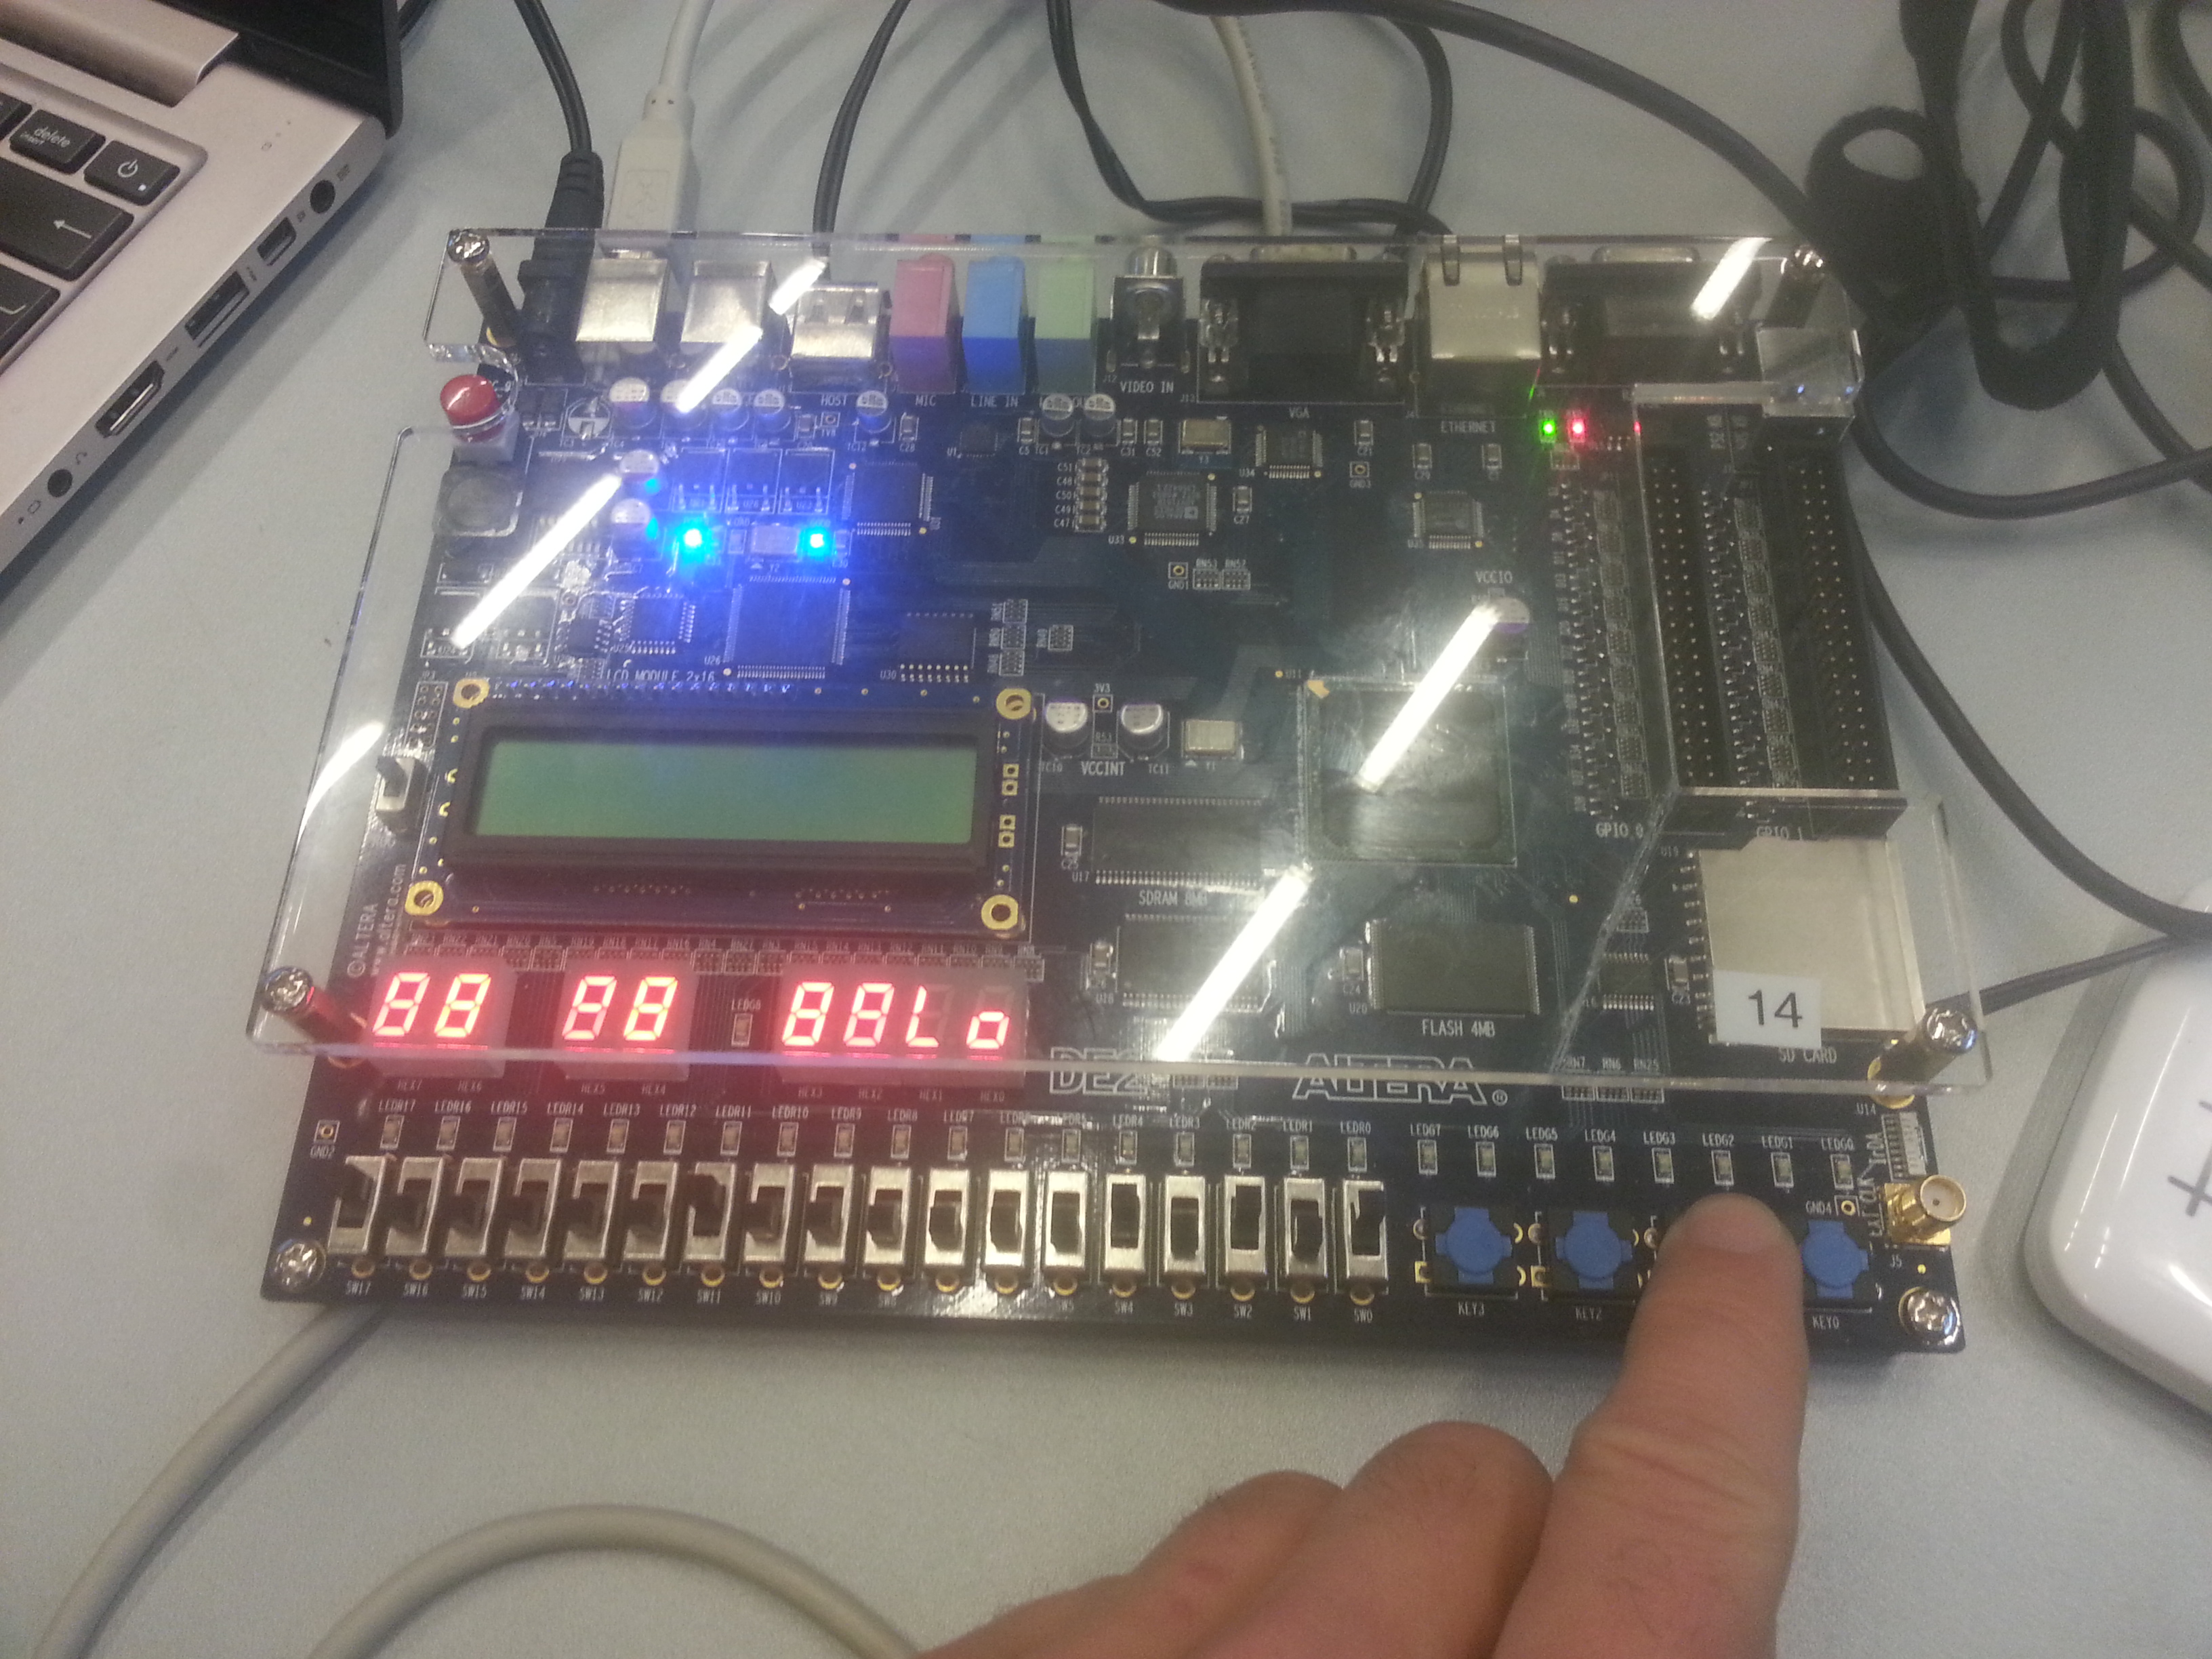
\includegraphics[scale=0.8]{pictures/Oevelse5/opg3/guess_try_lo.JPG}
		\caption{}
		\label{fig:GuessTryLo}
	\end{figure}
	\begin{figure}[h]
		\centering
		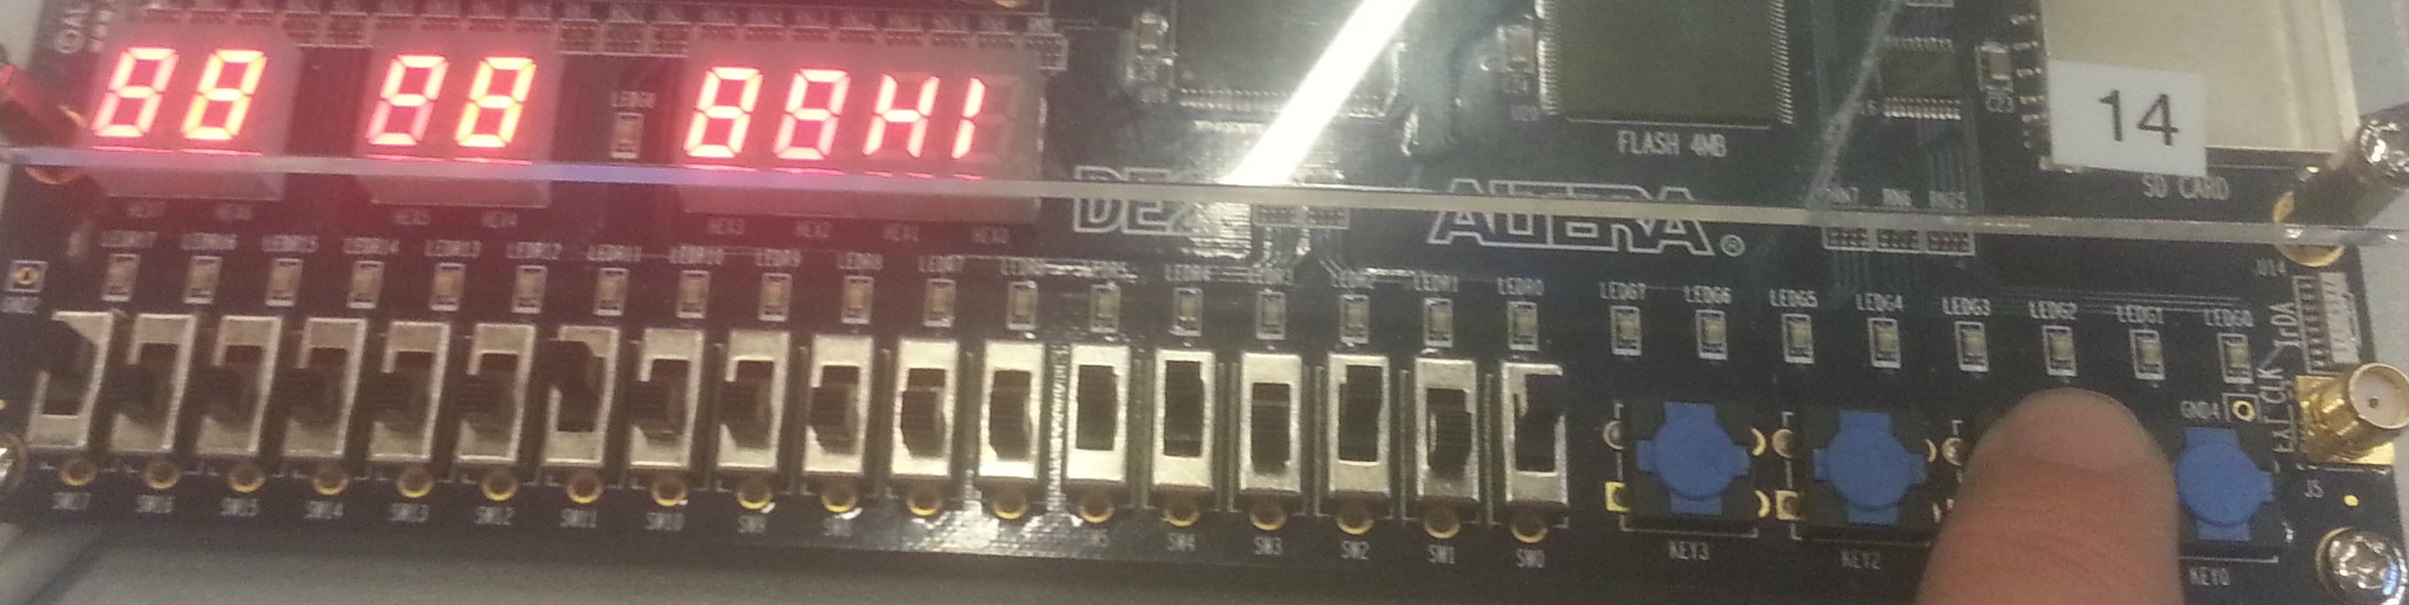
\includegraphics[scale=0.8]{pictures/Oevelse5/opg3/guess_try_hi.JPG}
		\caption{}
		\label{fig:GuessTryHi}
	\end{figure}
	\begin{figure}[h]
		\centering
		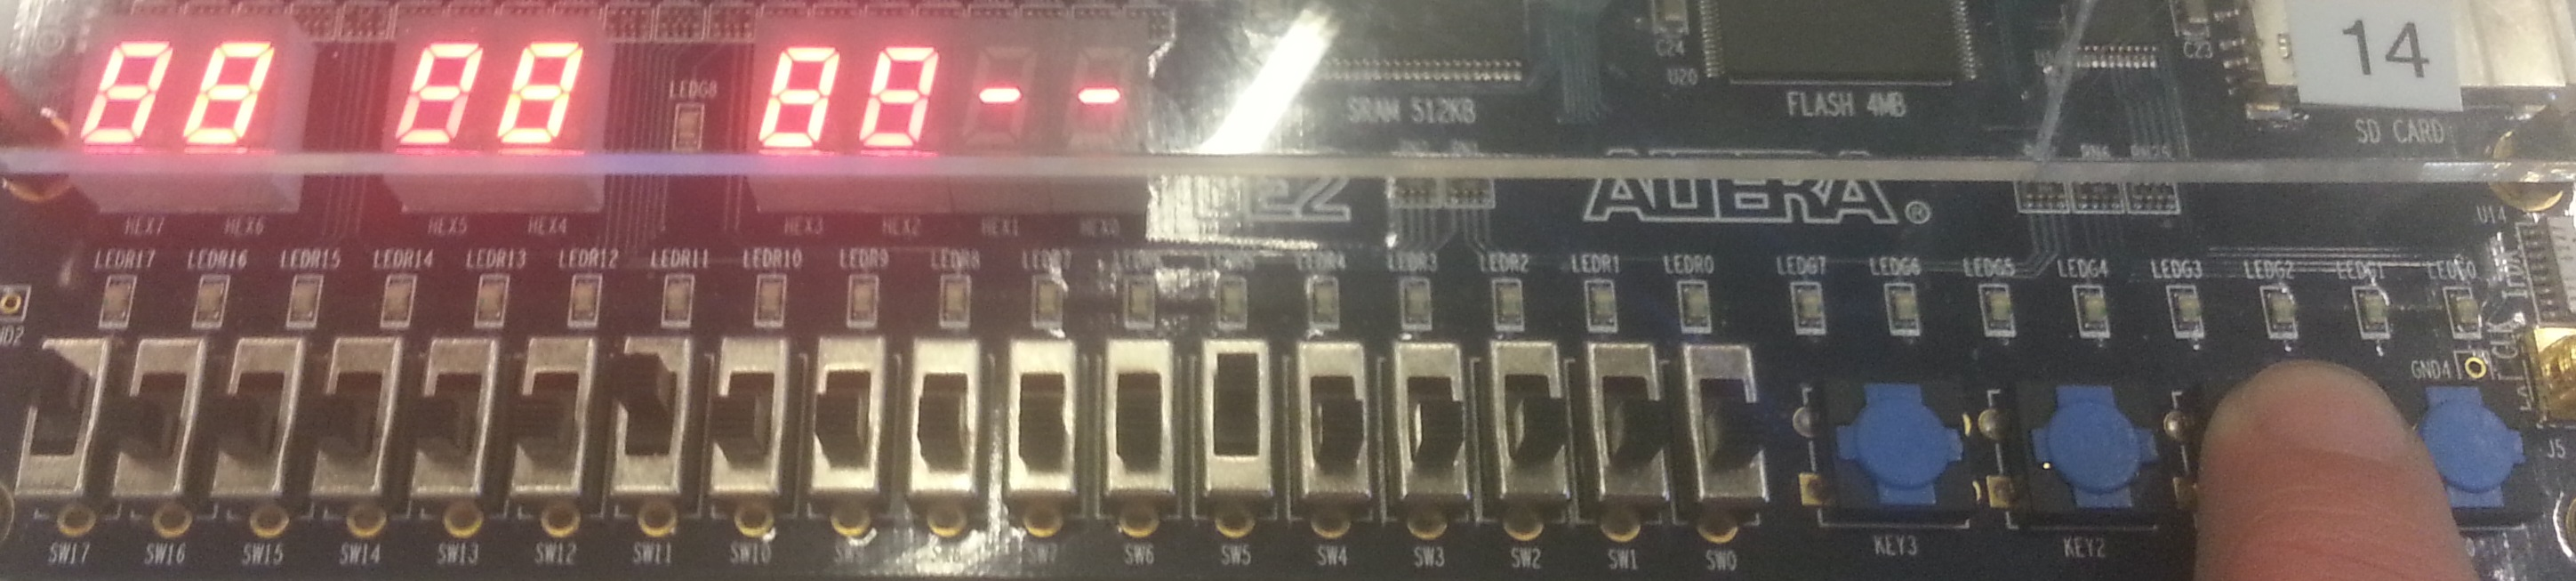
\includegraphics[scale=0.8]{pictures/Oevelse5/opg3/guess_try_ok.JPG}
		\caption{}
		\label{fig:GuessTryOk}
	\end{figure}
	\begin{figure}[h]
		\centering
		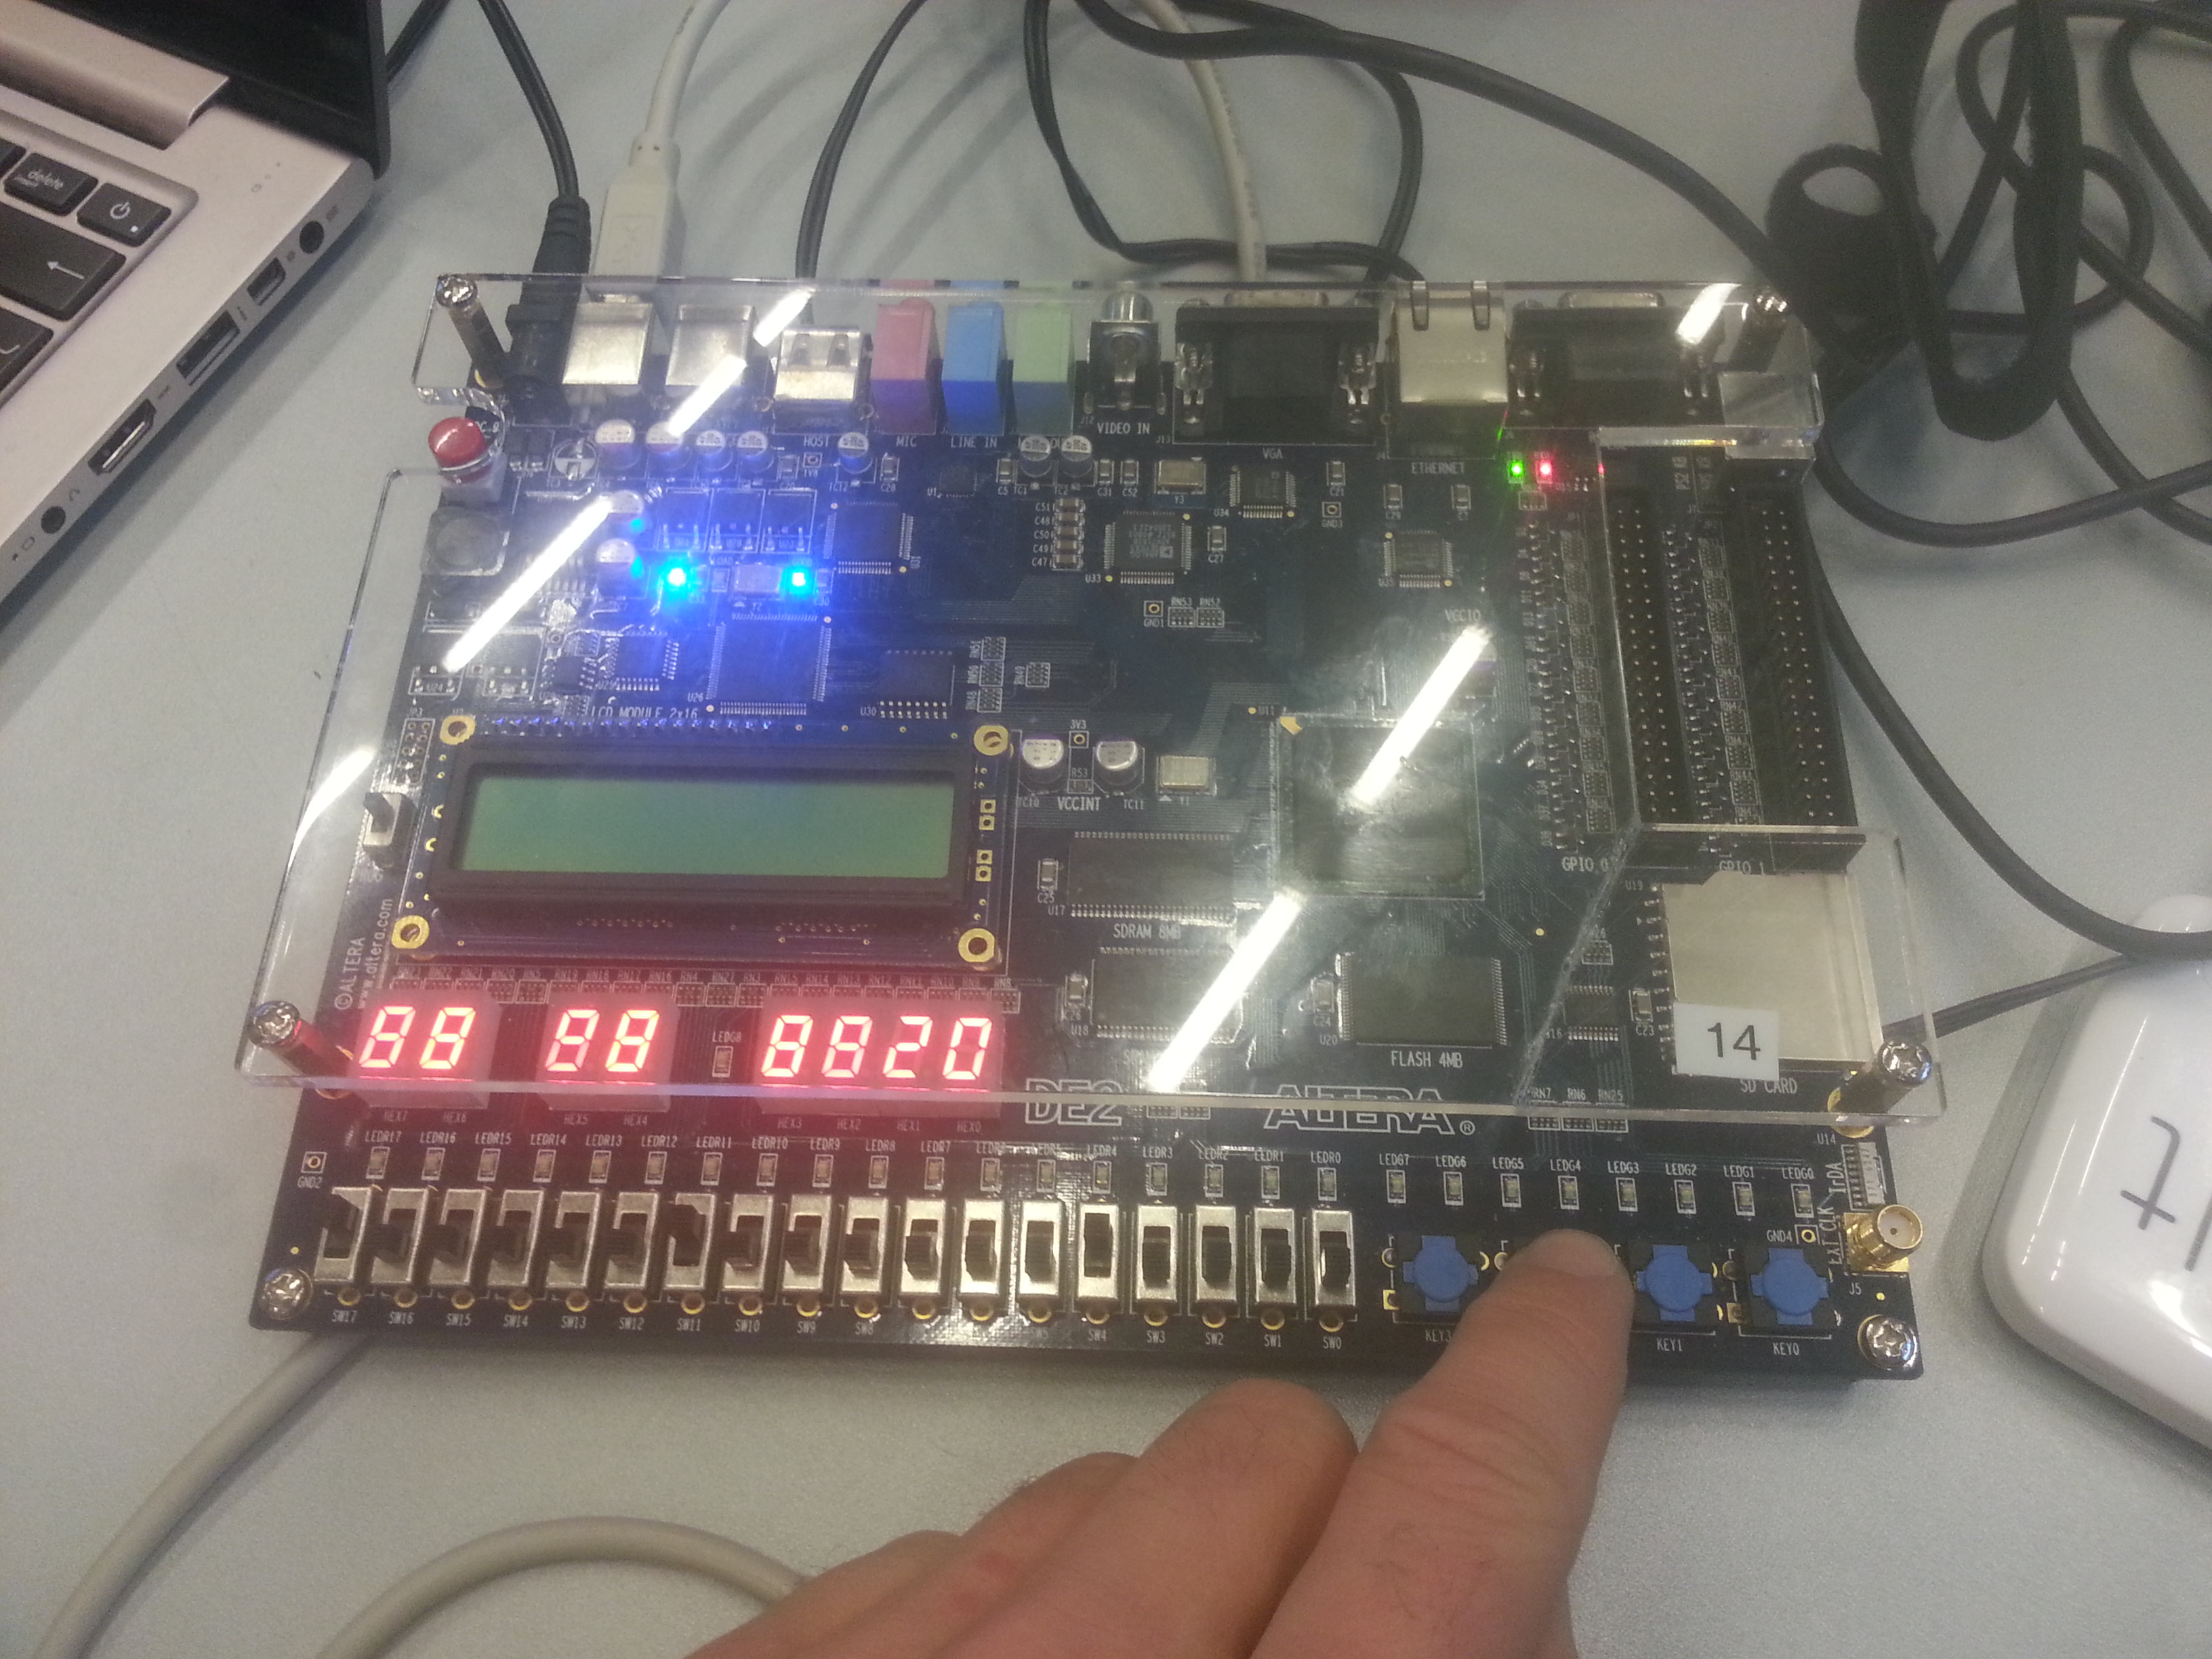
\includegraphics[scale=0.8]{pictures/Oevelse5/opg3/guess_show.JPG}
		\caption{}
		\label{fig:GuessShow}
	\end{figure}
		\item[1)]
		Vi skriver koden for vores Guessgame som det ses på figur \ref{lst:Guessgame}.\\
		\begin{lstlisting}[caption={Behavioral style kode for Guessgame},label={lst:Guessgame}]
		library ieee;
		use ieee.std_logic_1164.all;
		use ieee.numeric_std.all;
		
		entity guessgame is 
		port (input : in std_logic_vector(7 downto 0);
		set, show, try : in std_logic;
		seg1, seg10 : out std_logic_vector(6 downto 0));
		end guessgame;
		
		architecture game_process of guessgame is
		signal i_input10 : std_logic_vector(7 downto 4);
		signal i_input1 : std_logic_vector(3 downto 0);
		signal i_seg1, i_seg10 : std_logic_vector(3 downto 0);
		begin
		count: process (set, show, try)
		
		variable target : std_logic_vector(7 downto 0);
		
		begin
		
		--target := "00000000";
		
		if set = '0' then target := input;
		elsif show = '0' then 
		i_seg1 <= target(3 downto 0);
		i_seg10 <= target(7 downto 4);
		case i_seg1 is
		when "0000" => seg1 <= "0000001"; -- 0
		when "0001" => seg1 <= "1001111"; -- 1
		when "0010" => seg1 <= "0010010"; -- 2
		when "0011" => seg1 <= "0000110"; -- 3
		when "0100" => seg1 <= "1001100"; -- 4
		when "0101" => seg1 <= "0100100"; -- 5
		when "0110" => seg1 <= "0100000"; -- 6
		when "0111" => seg1 <= "0001111"; -- 7
		when "1000" => seg1 <= "0000000"; -- 8
		when "1001" => seg1 <= "0001100"; -- 9
		when "1010" => seg1 <= "0001000"; -- A
		when "1011" => seg1 <= "1100000"; -- B
		when "1100" => seg1 <= "0110001"; -- C
		when "1101" => seg1 <= "1000010"; -- D
		when "1110" => seg1 <= "0110000"; -- E
		when "1111" => seg1 <= "0111000"; -- F
		when others => seg1 <= "1111111"; -- Slukket
		end case;
		case i_seg10 is
		when "0000" => seg10 <= "0000001"; -- 0
		when "0001" => seg10 <= "1001111"; -- 1
		when "0010" => seg10 <= "0010010"; -- 2
		when "0011" => seg10 <= "0000110"; -- 3
		when "0100" => seg10 <= "1001100"; -- 4
		when "0101" => seg10 <= "0100100"; -- 5
		when "0110" => seg10 <= "0100000"; -- 6
		when "0111" => seg10 <= "0001111"; -- 7
		when "1000" => seg10	<= "0000000"; -- 8
		when "1001" => seg10	<= "0001100"; -- 9
		when "1010" => seg10 <= "0001000"; -- A
		when "1011" => seg10 <= "1100000"; -- B
		when "1100" => seg10 <= "0110001"; -- C
		when "1101" => seg10	<= "1000010"; -- D
		when "1110" => seg10 <= "0110000"; -- E
		when "1111" => seg10 <= "0111000"; -- F
		when others => seg10 <= "1111111"; -- Slukket
		end case;
		elsif try = '0' then 
		if input > target then --output Hi
		seg10 <= "1001000"; 
		seg1 <= "1111001";
		elsif input < target then -- output Lo
		seg10 <= "1110001"; 
		seg1 <= "1100010";
		elsif input = target then -- output --
		seg10 <= "1111110"; 
		seg1 <= "1111110";
		end if;
		elsif set = '1' and show = '1' and try = '1' then 
		i_input10 <= input(7 downto 4); 
		i_input1 <= input(3 downto 0);
		case i_input1 is
		when "0000" => seg1 <= "0000001"; -- 0
		when "0001" => seg1 <= "1001111"; -- 1
		when "0010" => seg1 <= "0010010"; -- 2
		when "0011" => seg1 <= "0000110"; -- 3
		when "0100" => seg1 <= "1001100"; -- 4
		when "0101" => seg1 <= "0100100"; -- 5
		when "0110" => seg1 <= "0100000"; -- 6
		when "0111" => seg1 <= "0001111"; -- 7
		when "1000" => seg1 <= "0000000"; -- 8
		when "1001" => seg1 <= "0001100"; -- 9
		when "1010" => seg1 <= "0001000"; -- A
		when "1011" => seg1 <= "1100000"; -- B
		when "1100" => seg1 <= "0110001"; -- C
		when "1101" => seg1 <= "1000010"; -- D
		when "1110" => seg1 <= "0110000"; -- E
		when "1111" => seg1 <= "0111000"; -- F
		when others => seg1 <= "1111111"; -- Slukket
		end case;
		
		case i_input10 is
		when "0000" => seg10 <= "0000001"; -- 0
		when "0001" => seg10 <= "1001111"; -- 1
		when "0010" => seg10 <= "0010010"; -- 2
		when "0011" => seg10 <= "0000110"; -- 3
		when "0100" => seg10 <= "1001100"; -- 4
		when "0101" => seg10 <= "0100100"; -- 5
		when "0110" => seg10 <= "0100000"; -- 6
		when "0111" => seg10 <= "0001111"; -- 7
		when "1000" => seg10 <= "0000000"; -- 8
		when "1001" => seg10 <= "0001100"; -- 9
		when "1010" => seg10 <= "0001000"; -- A
		when "1011" => seg10 <= "1100000"; -- B
		when "1100" => seg10 <= "0110001"; -- C
		when "1101" => seg10 <= "1000010"; -- D
		when "1110" => seg10 <= "0110000"; -- E
		when "1111" => seg10 <= "0111000"; -- F
		when others => seg10 <= "1111111"; -- Slukket
		end case;
		end if;
		end process count;
		end game_process;
		
		
		\end{lstlisting}
		\item[2)]
		Vi downloader programmet til vores DE2-board, hvor SW[0-3] vises på HEX0, SW[4-7] vises på HEX1, KEY3 = set, KEY2 = show og KEY1 = try. \\
		\begin{figure}[h]
			\centering
			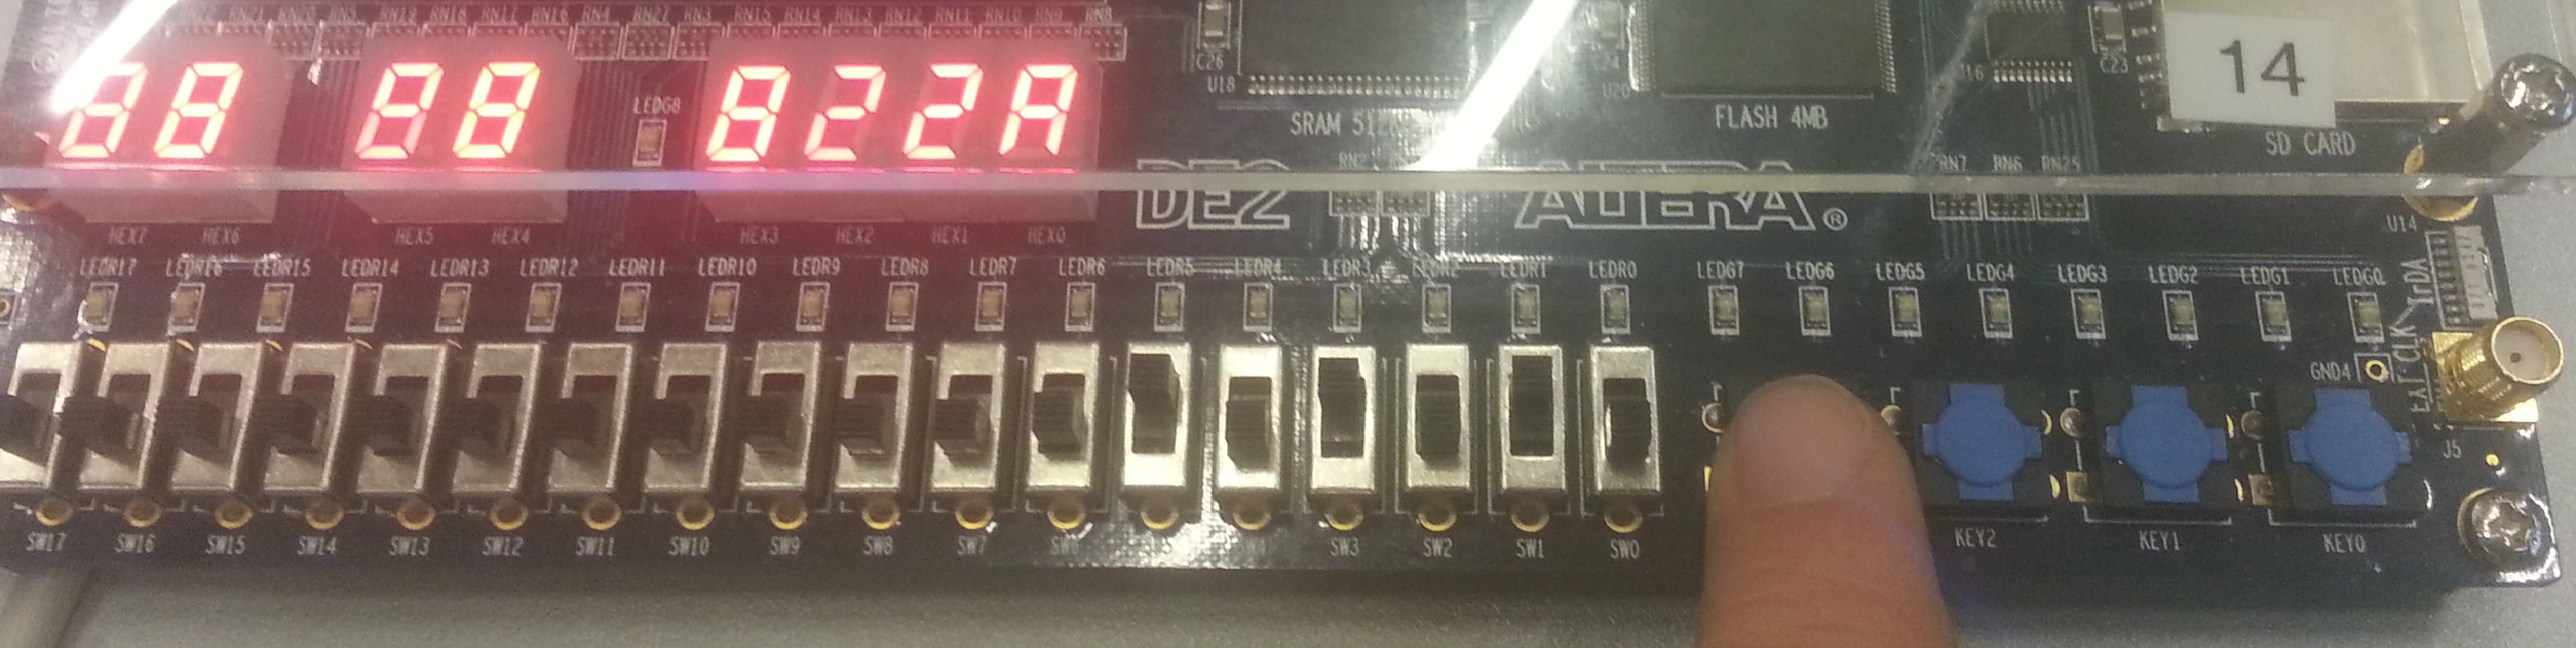
\includegraphics[scale=0.8]{pictures/Oevelse5/opg3/guess_2p_set.JPG}
			\caption{}
			\label{fig:Guess2pSet}
		\end{figure}
		\begin{figure}[h]
			\centering
			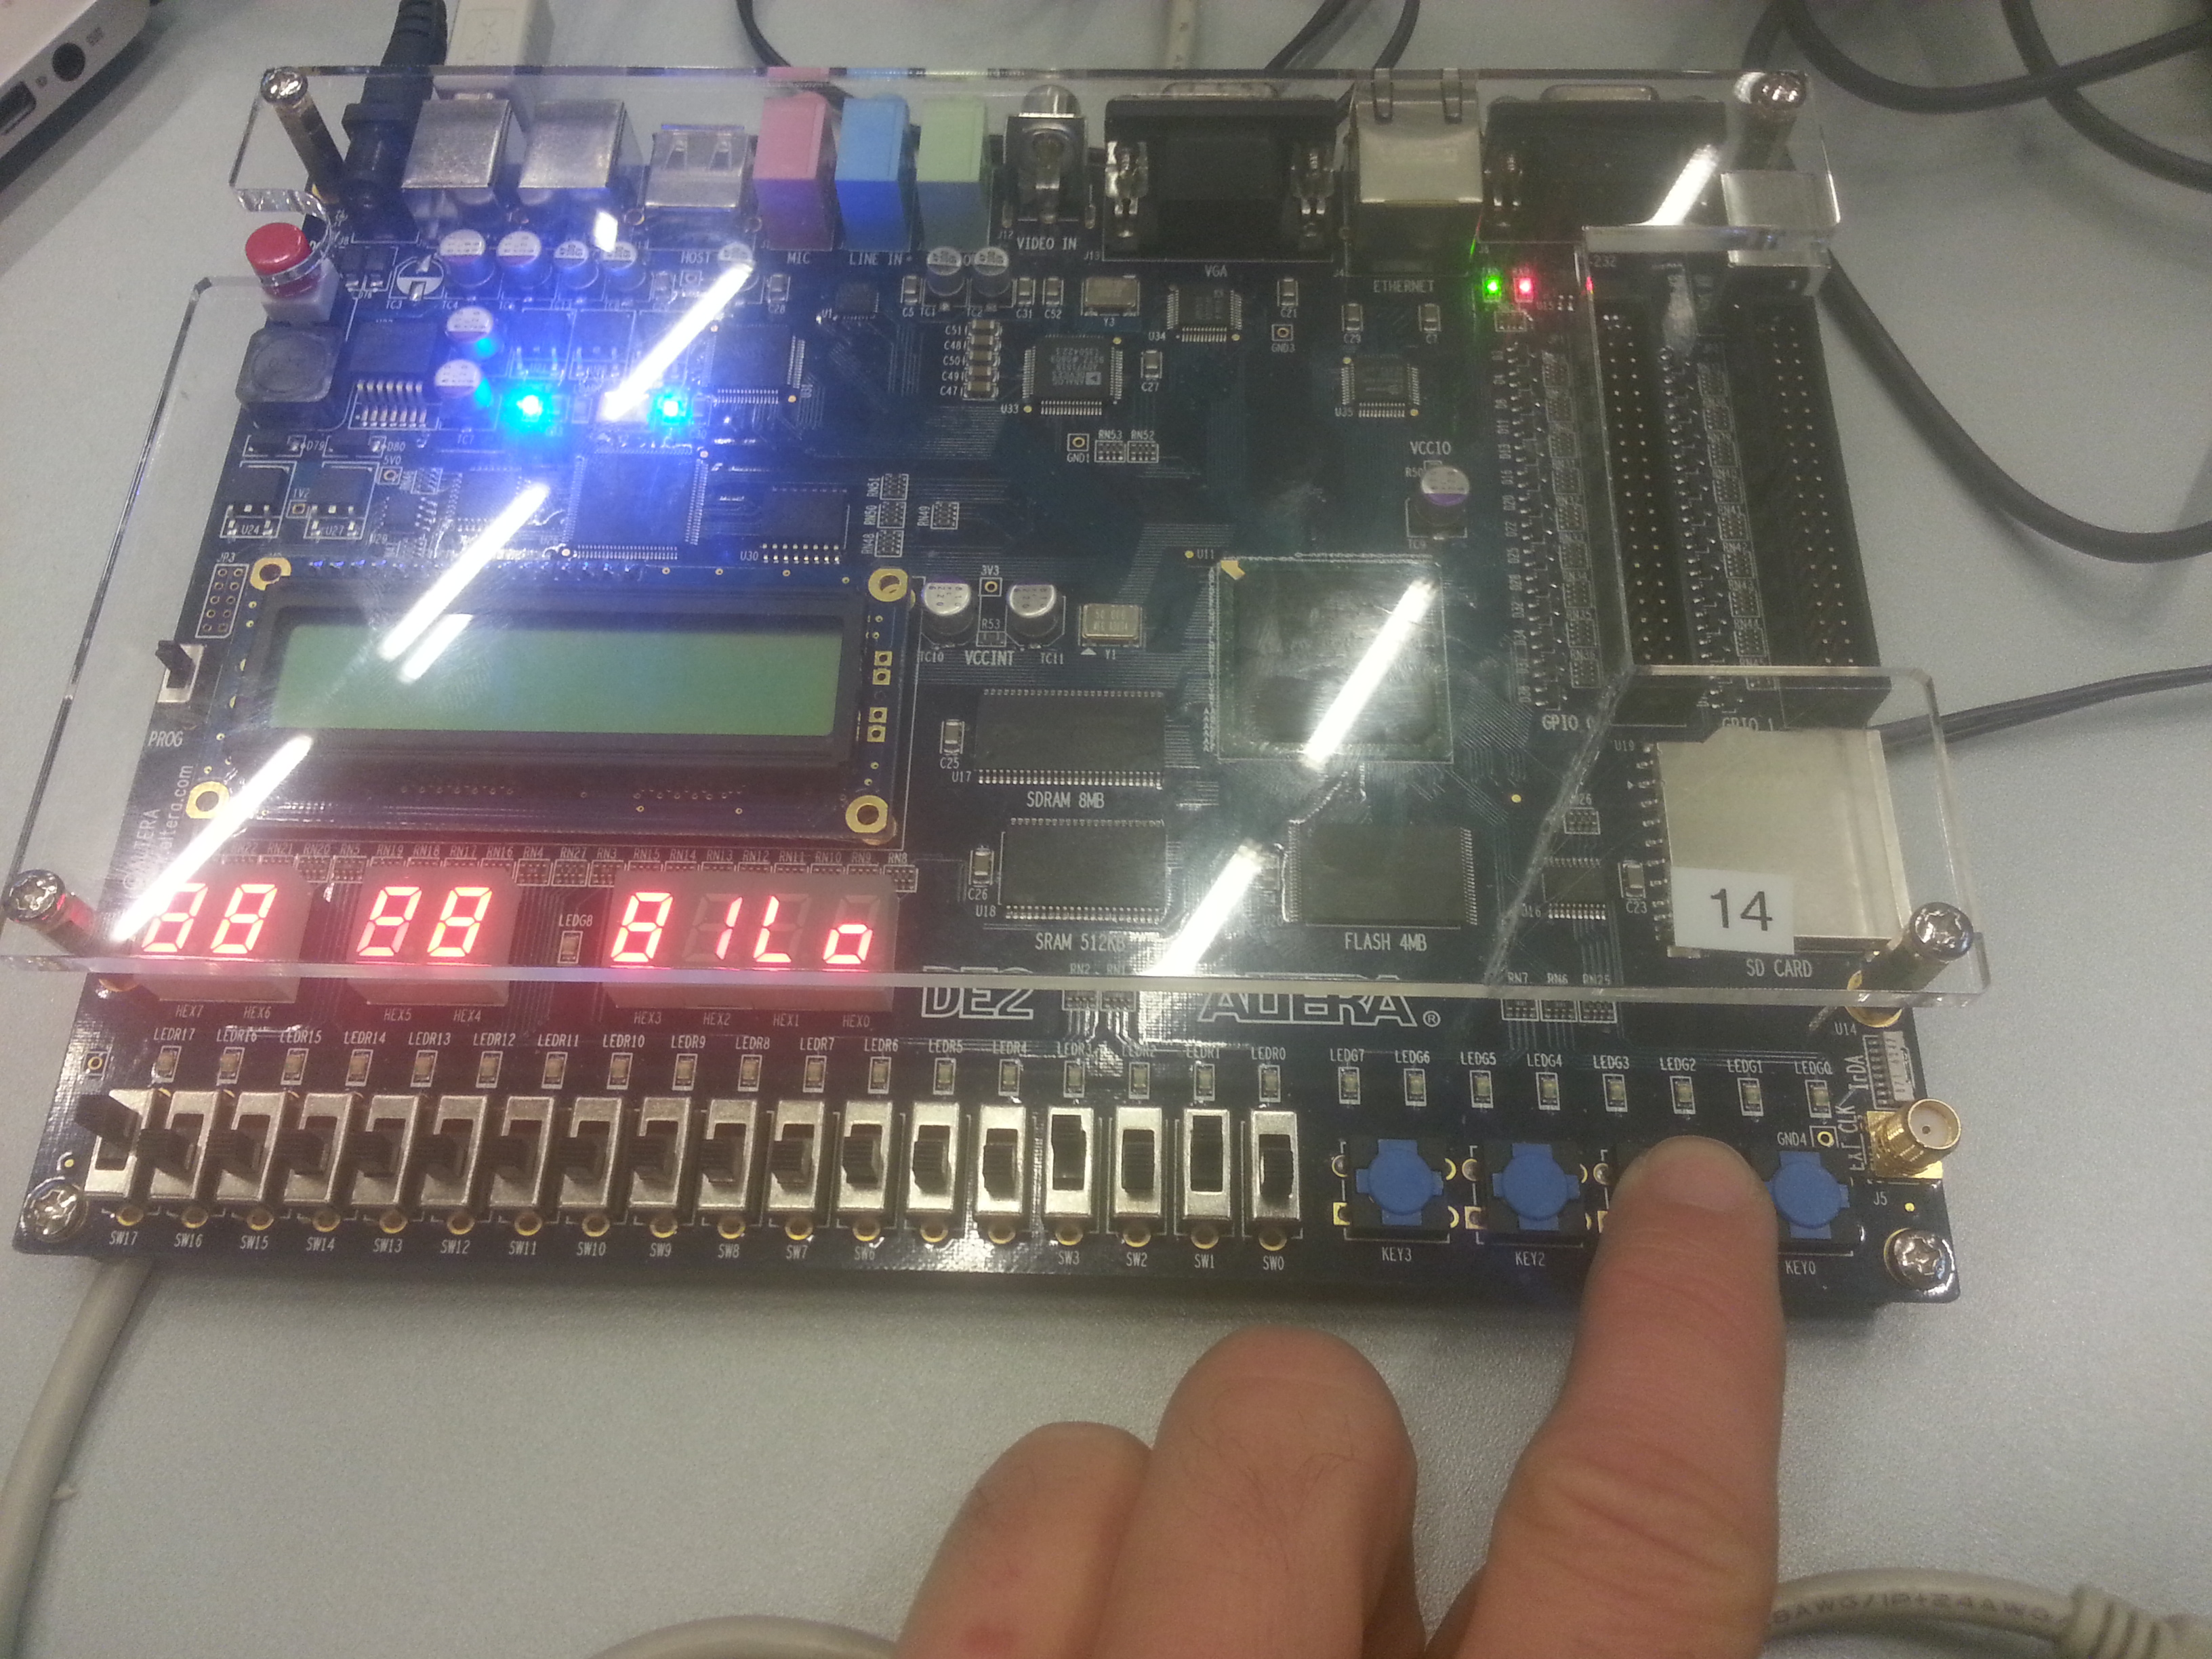
\includegraphics[scale=0.8]{pictures/Oevelse5/opg3/guess_2p_try_lo.JPG}
			\caption{}
			\label{fig:Guess2pTryLo}
		\end{figure}
		\begin{figure}[h]
			\centering
			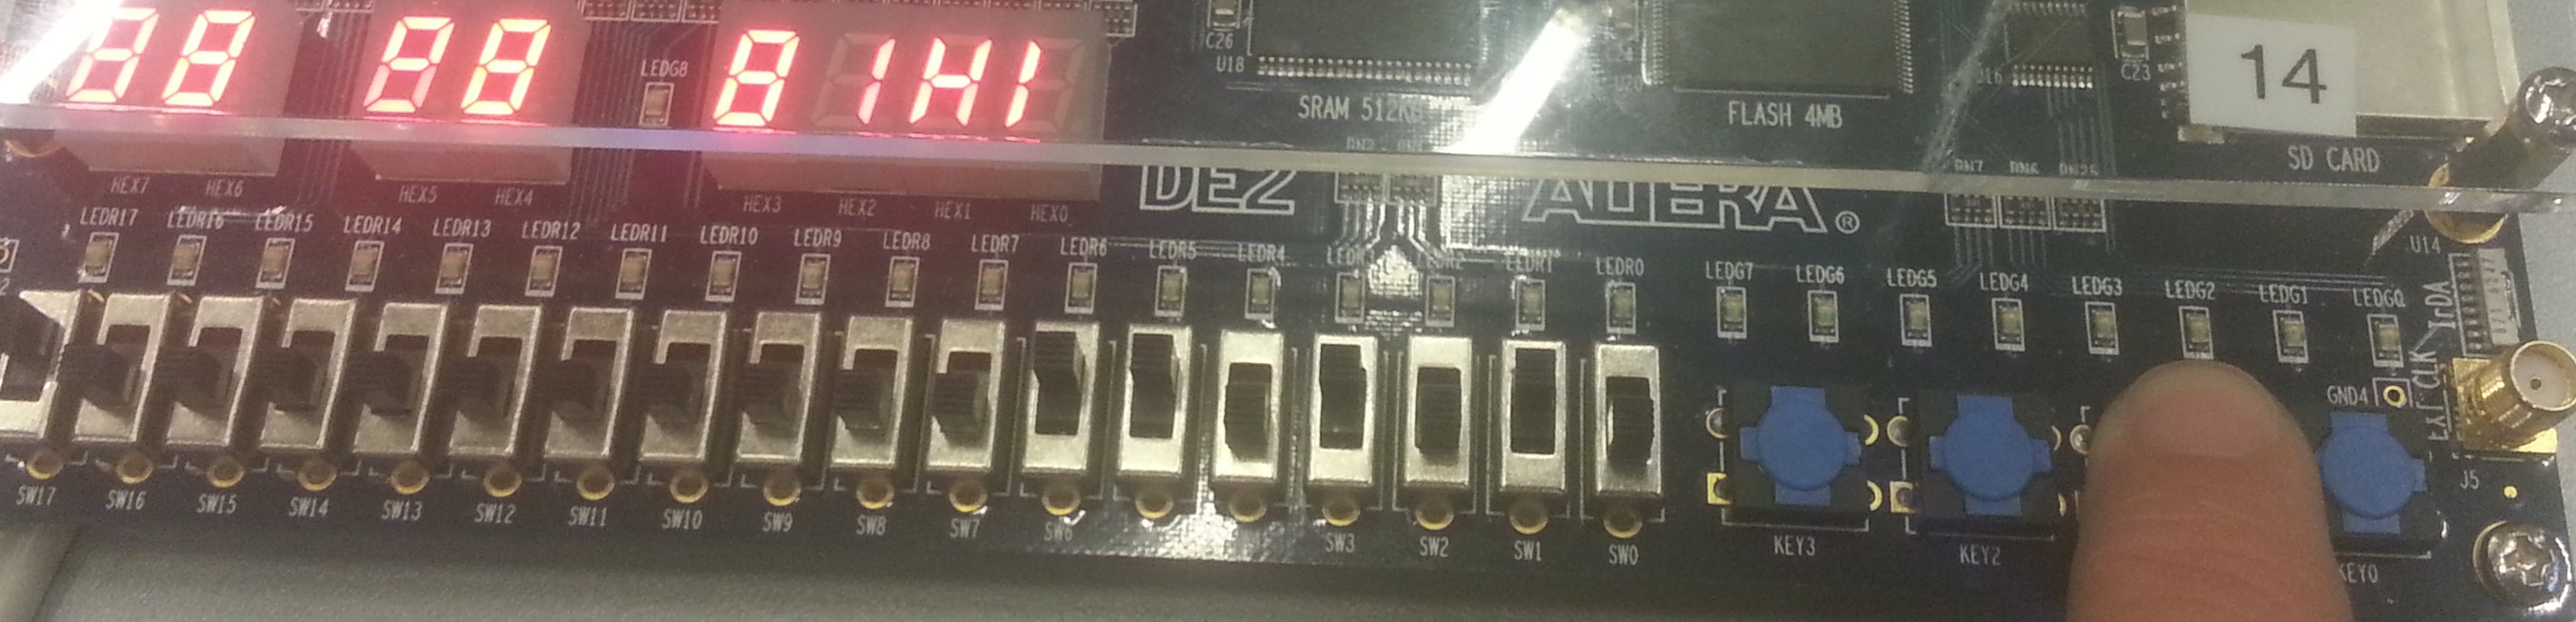
\includegraphics[scale=0.8]{pictures/Oevelse5/opg3/guess_2p_try_hi.JPG}
			\caption{}
			\label{fig:Guess2pTryHi}
		\end{figure}
		\begin{figure}[h]
			\centering
			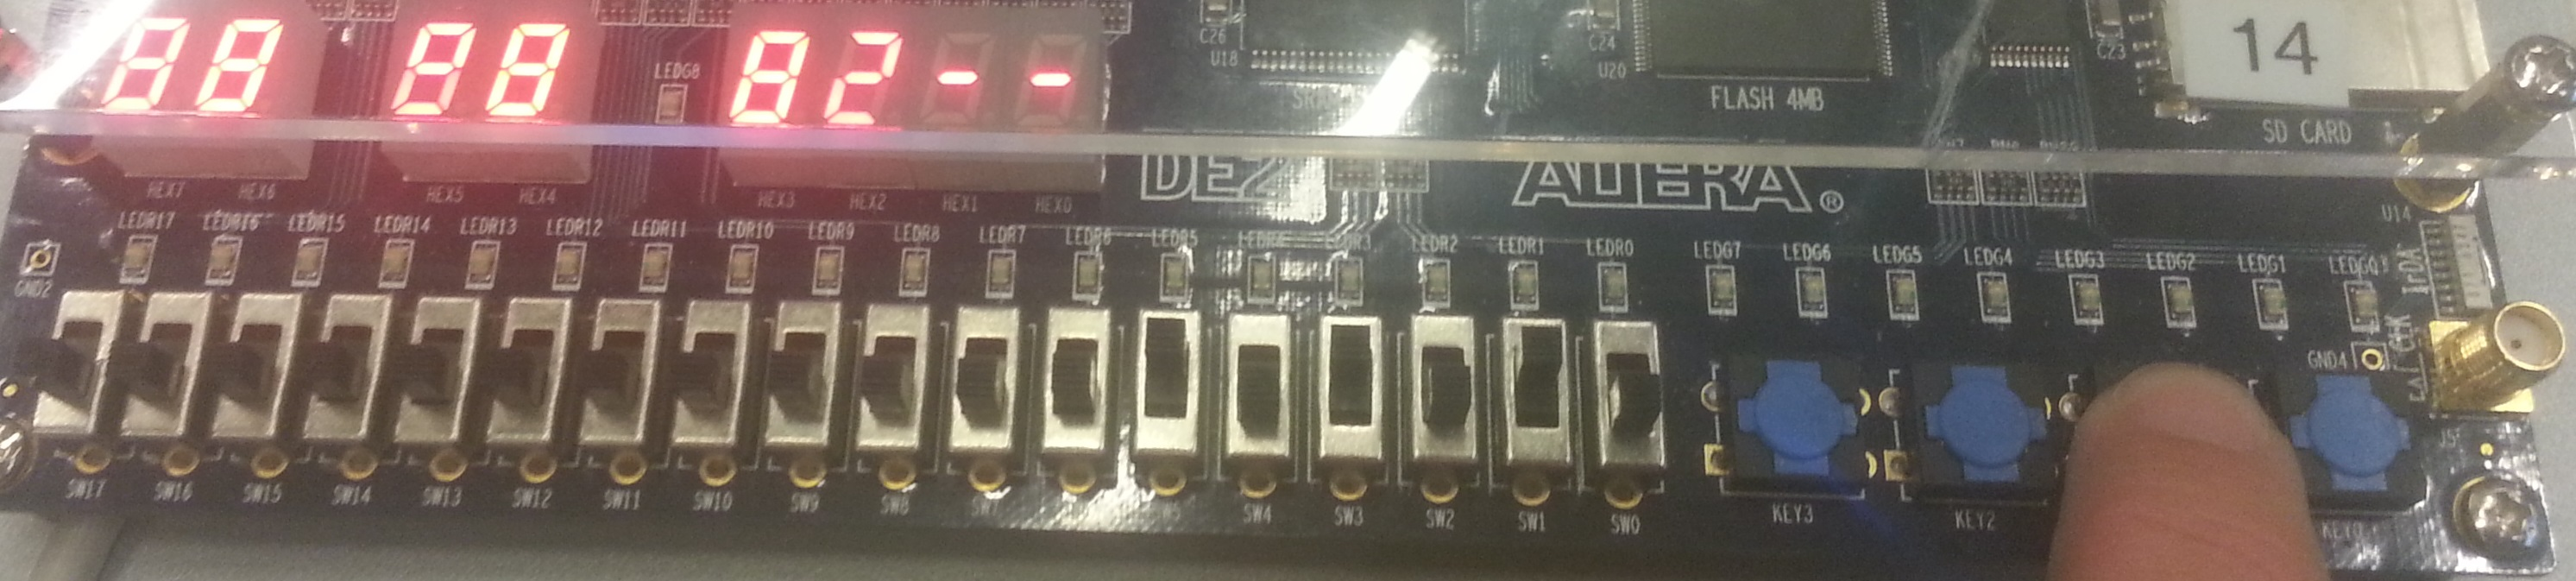
\includegraphics[scale=0.8]{pictures/Oevelse5/opg3/guess_2p_try_ok.JPG}
			\caption{}
			\label{fig:Guess2pTryOk}
		\end{figure}
		\begin{figure}[h]
			\centering
			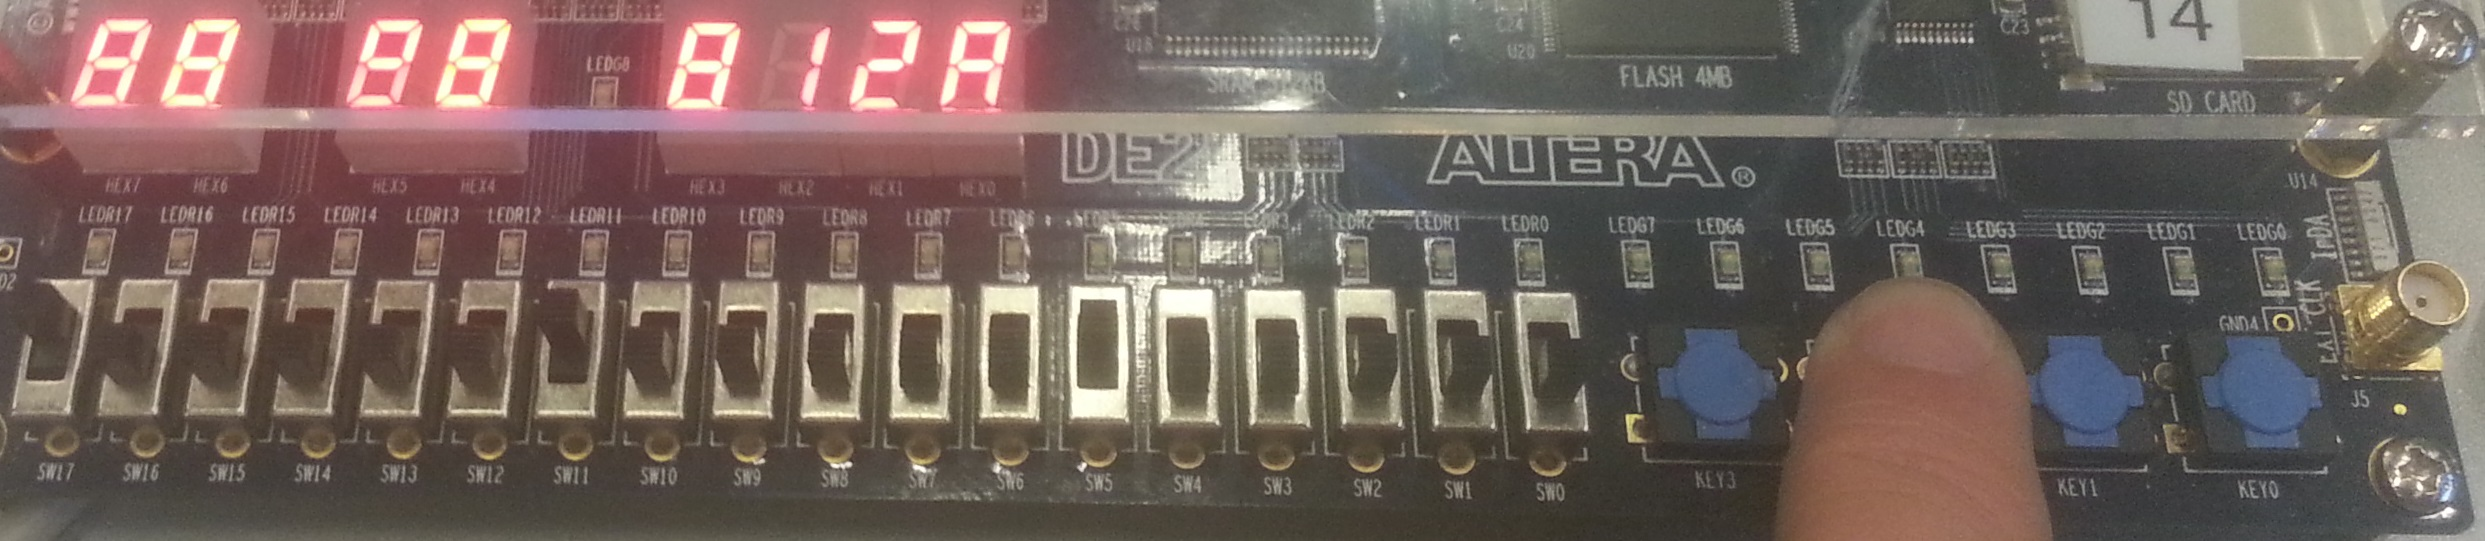
\includegraphics[scale=0.8]{pictures/Oevelse5/opg3/guess_2p_show.JPG}
			\caption{}
			\label{fig:Guess2pShow}
		\end{figure}
\end{enumerate}